\apendice{Especificación de Requisitos}

Este anexo ha sido adaptado con la información que define el desarrollo realizado, ya que, aunque no se trata de un sistema con interacción directa con el usuario, la solución propuesta incluye funcionalidades software.


En este proyecto existe una lógica funcional bien definida, estructurada en tareas del firmware, que interactúa tanto con los sensores físicos como con el usuario investigador a través del puerto serie. Por ello, se ha definido un caso de uso técnico que representa el comportamiento del sistema en relación con la adquisición, procesamiento y extracción de datos biomédicos.

\section{Diagrama de casos de uso}

\begin{figure}[H]
    \centering
    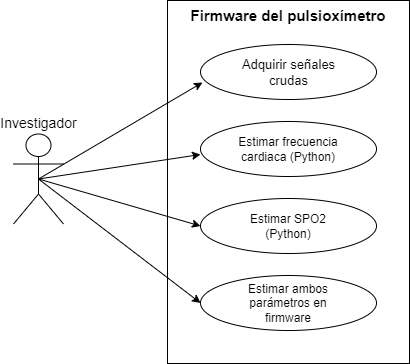
\includegraphics[scale =0.43]{img/casodeuso1.png}
    \caption{CU-1. \textit{Elaboración propia}}
    \label{fig:casos_uso}
\end{figure}



\section{Explicación casos de uso.}

\begin{table}[H]
	\centering
	\begin{tabularx}{\linewidth}{ p{0.21\columnwidth} p{0.71\columnwidth} }
		\toprule
		\textbf{CU-1}    & \textbf{Adquirir señales crudas} \\
		\toprule
		\textbf{Versión}              & 1.0 \\
		\textbf{Autor}                & Elena Ruiz \\
		\textbf{Descripción}          & El sistema adquiere señales fotopletismográficas crudas del sensor U401-D a través del AFE4490 y las envía al PC mediante comunicación serie. Los datos son almacenados en formato csv para su posterior análisis.\\
		\textbf{Precondición}         & El sensor debe estar correctamente conectado y alimentado. El microcontrolador debe haber iniciado correctamente el firmware. \\
		\textbf{Acciones}             &
		\begin{enumerate}
			\item Conectar los elementos necesarios del sistema hardware.
			\item Asegurar la correcta conexión y el reconocimiento de la placa por el ordenador.
			\item Registrar un log individual a la vez que se están midiendo los valores con un pulsioximetro externo de referencia.
			\item Guardar los datos en un archivo CSV mediante un script en Python.
		\end{enumerate} \\
		\textbf{Postcondición}        & Se genera un archivo CSV con las señales crudas. \\
		\textbf{Excepciones}          & Pérdida de comunicación serie, fallo en la alimentación del sensor, datos corruptos. \\
		\textbf{Importancia}          & Alta \\
		\bottomrule
	\end{tabularx}
	\caption{CU-1 Adquirir señales crudas. \textit{Elaboración propia.}}
\end{table}


\begin{table}[H]
	\centering
	\begin{tabularx}{\linewidth}{ p{0.21\columnwidth} p{0.71\columnwidth} }
		\toprule
		\textbf{CU-2}    & \textbf{Estimar frecuencia cardiaca (Python)} \\
		\toprule
		\textbf{Versión}              & 1.0 \\
		\textbf{Autor}                & Elena Ruiz \\
		\textbf{Descripción}          & El sistema procesa la señal PPG en formato .csv para detectar picos y calcular la frecuencia cardíaca en tiempo no real utilizando scripts en Python. \\
		\textbf{Precondición}         & El archivo CSV con datos crudos debe existir y estar completo. \\
		\textbf{Acciones}             &
		\begin{enumerate}
			\item Cargar el archivo CSV con las señales IR y/o RED.
			\item Aplicar filtrado.
			\item Detectar picos correspondientes a los latidos.
			\item Calcular la frecuencia cardíaca media (en BPM).
		\end{enumerate} \\
		\textbf{Postcondición}        & Se obtiene un valor estimado de frecuencia cardíaca, que puede compararse con la referencia externa. Los algoritmos que mejor resultados ofrecen son estudiados posteriormente para ser implementados en el firmware.\\
		\textbf{Excepciones}          & Señal demasiado ruidosa, número insuficiente de picos, error de formato en CSV. \\
		\textbf{Importancia}          & Alta \\
		\bottomrule
	\end{tabularx}
	\caption{CU-2 Estimar frecuencia cardiaca (Python). \textit{Elaboración propia.}}
\end{table}

\begin{table}[H]
	\centering
	\begin{tabularx}{\linewidth}{ p{0.21\columnwidth} p{0.71\columnwidth} }
		\toprule
		\textbf{CU-3}    & \textbf{Estimar SpO$_2$ (Python)} \\
		\toprule
		\textbf{Versión}              & 1.0 \\
		\textbf{Autor}                & Elena Ruiz \\
		\textbf{Descripción}          & El sistema calcula la saturación de oxígeno estimada a partir del cociente de las señales PPG. \\
		\textbf{Precondición}         & El archivo CSV debe contener las señales correctamente sincronizadas y calibradas. \\
		\textbf{Acciones}             &
		\begin{enumerate}
			\item Cargar y recortar las señales.
			\item Aplicar filtros a las señales RED e IR.
			\item Calcular componentes AC y DC mediante media y picos.
			\item Obtener el índice R = (ACred/DCred) / (ACir/DCir).
			\item Estimar SpO$_2$ con tabla LUT o regresión calibrada.
		\end{enumerate} \\
		\textbf{Postcondición}        & Se muestra el valor estimado de SpO$_2$ para la sesión analizada. \\
		\textbf{Excepciones}          & Cálculo inválido por baja perfusión, señales ruidosas o relación R fuera del rango. Los algoritmos que mejor resultados ofrecen son estudiados posteriormente para ser implementados en el firmware. \\
		\textbf{Importancia}          & Alta \\
		\bottomrule
	\end{tabularx}
	\caption{CU-3 Estimar SpO$_2$ (Python). \textit{Elaboración propia.}}
\end{table}

\begin{table}[H]
	\centering
	\begin{tabularx}{\linewidth}{ p{0.21\columnwidth} p{0.71\columnwidth} }
		\toprule
		\textbf{CU-4}    & \textbf{Estimar frecuencia cardíaca y SpO$_2$ (firmware)} \\
		\toprule
		\textbf{Versión}              & 1.0 \\
		\textbf{Autor}                & Elena Ruiz \\
		\textbf{Descripción}          & El firmware del microcontrolador procesa las señales PPG en tiempo real para calcular la frecuencia cardíaca y la saturación de oxígeno utilizando los algoritmos previamente probados en entorno Python. \\
		\textbf{Precondición}         & Sensor y AFE correctamente inicializados, condiciones de señal adecuadas, adquisición continua activada. \\
		\textbf{Acciones}             &
		\begin{enumerate}
			\item Leer muestras IR y RED desde el AFE4490.
			\item Aplicar los algoritmos estudiados que han sido implementados en C++.
			\item Mostrar Frecuencia cardiaca y SpO$_2$ por UART al PC.
            \item Comparar resultado en tiempo real con un pulsioxímetro externo de referencia.
		\end{enumerate} \\
		\textbf{Postcondición}        & Se envían los valores estimados de HR y SpO$_2$ al sistema de monitorización y/o se muestran en pantalla. \\
		\textbf{Excepciones}          & Datos erróneos por movimiento, baja señal o demasiada intensidad de luz.\\
		\textbf{Importancia}          & Muy alta \\
		\bottomrule
	\end{tabularx}
	\caption{CU-4 Estimar frecuencia cardíaca y SpO$_2$ (firmware). \textit{Elaboración propia.}}
\end{table}


\section{Prototipos de interfaz o interacción con el proyecto.}

El sistema implementado, en el grado de desarrollo en el que se encuentra, no dispone de una interfaz gráfica de usuario avanzada. Sin embargo, se han considerado dos formas de interacción o visualización con el sistema:

\subsection{Salida por terminal serie}

Durante el desarrollo y las pruebas del sistema, la información de frecuencia cardíaca y saturación de oxígeno estimada en firmware se muestra por consola a través del puerto serie, utilizando el monitor serial de Visual Studio Code. En la Figura \ref{fig: Captura_firmware} puede observarse una captura de la salida real del sistema, donde se visualizan los valores estimados por el microcontrolador en tiempo real.

\begin{figure}[H]
    \centering
    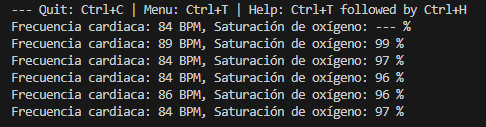
\includegraphics[width=0.7\textwidth]{img/Captura_firmware.png}
    \caption{Salida de datos del pulsioxímetro por consola serie (Visual Studio Code). \textit{Elaboración propia.}}
    \label{fig: Captura_firmware}
\end{figure}

\subsection{Interfaz en pantalla integrada (prototipo simulado)}

Idealmente, los valores deberían visualizarse en el display integrado en la incubadora neonatal (pantalla TFT). Sin embargo, por limitaciones técnicas y de tiempo, esta parte no ha podido completarse durante el desarrollo del TFG. Para reflejar la intención de diseño, se ha generado un prototipo gráfico (Figura \ref{fig:display_mockup}) que representa cómo se espera mostrar la información final en el dispositivo. En dicha interfaz se muestran los valores de temperatura, humedad, SpO$_2$ y frecuencia cardíaca en un formato claro, accesible y compatible con el resto de la interfaz de la incubadora.

\begin{figure}[H]
    \centering
    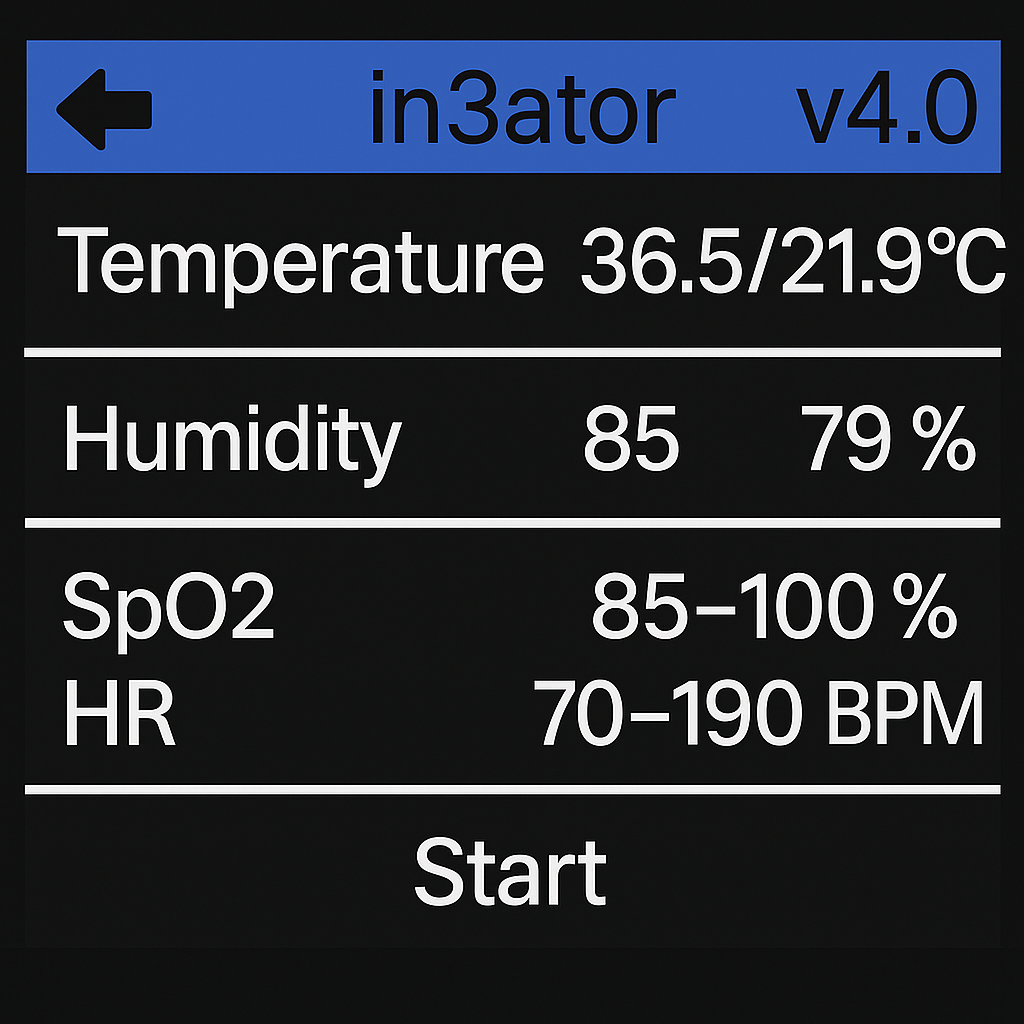
\includegraphics[width=0.3\textwidth]{img/display.png}
    \caption{Prototipo simulado de la interfaz final en el display de la incubadora. \textit{Elaboración propia.}}
    \label{fig:display_mockup}
\end{figure}






